\subsection{Formulation of the inverse problem}
\label{subsec:intro:formalism}
The \emph{forward problem} can be mathematically defined as the process of finding a mapping, $\mathcal{M}$, from the set of all possible parameters, $\mathcal{X}$, to the set of all possible measurement results, $\mathcal{Y}$, in order to predict the result of any possible measurement. This can be represented as: $\mathcal{M}: \mathcal{X} \mapsto \mathcal{Y}$. The \emph{inverse problem} is the opposite of the forward problem, which involves specifying the mapping $\mathcal{M}^{-1}: \mathcal{Y}\ \mapsto \textbf{P}\left(\mathcal{X}\right)$ explicitly from measurement results.

The problem is easy to define, but very hard to solve for practical material science application. The reasons are two-fold. Firstly, mapping $\mathcal{M}$ is a sophisticated computer program not susceptible to analytical tools. Most of them are even not differentiable. And almost all computational methods rely on approximation, leading to systematic uncertainty. Secondly, sometimes event a computer simulation is unfeasible, forcing us to rely on a data sample $\mathcal{D}$. Experimental data are are susceptible to measurement error. A \emph{surrogate model} $\widehat{\mathcal{M}}$ is a common solution to these problems. It approximates the forward model $\mathcal{M}$, but is easier to analyse, usually less computationally intensive and differentiable.

The use of exact inversion methods is often impractical in real-world scenarios due to their reliance on idealized assumptions which at not fulfilled for practical cases. These methods are also often unstable, and the goal in many inverse problems is to find a continuous mapping of the space variables. However, in practice, the amount of data available for reconstructing this mapping is limited, and the data may not contain sufficient information to accurately reconstruct the model \cite{sniederLinearNonlinearInverse2000}.

Practical inverse problems usually involve additional steps depicted in figure~\ref{fig:inverse_problem}: 
\begin{enumerate*}[label=(\alph*)]
    \item estimating a surrogate model, denoted as $\widehat{\mathcal{M}}$, from the data $\mathcal{D}$; and
    \item evaluating the accuracy of the estimated surrogate model with respect to the true model $\mathcal{M}$, which is known as the appraisal problem \cite{sniederLinearNonlinearInverse2000}.
\end{enumerate*}

\begin{figure}[htp]
\centering


\tikzset{every picture/.style={line width=0.75pt}} %set default line width to 0.75pt        

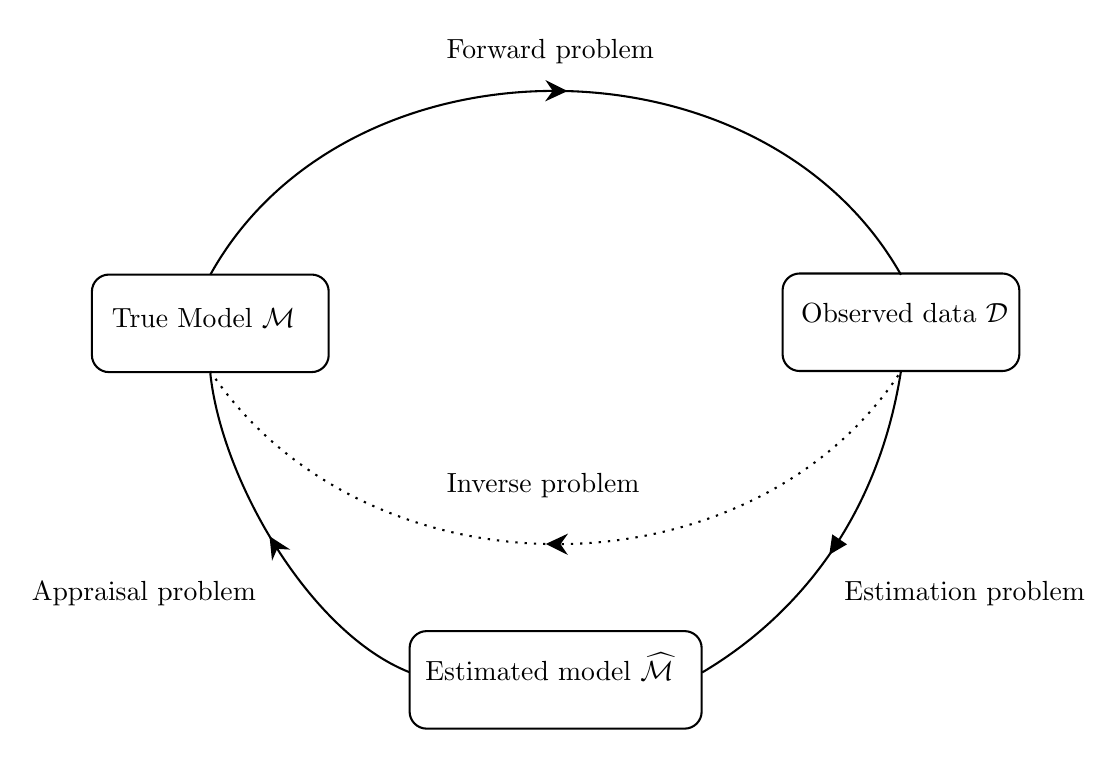
\begin{tikzpicture}[x=0.75pt,y=0.75pt,yscale=-1,xscale=1]
%uncomment if require: \path (0,366); %set diagram left start at 0, and has height of 366

%Flowchart: Alternative Process [id:dp654266910257798] 
\draw   (227.91,129.45) .. controls (227.91,124.91) and (231.59,121.23) .. (236.13,121.23) -- (333.77,121.23) .. controls (338.31,121.23) and (342,124.91) .. (342,129.45) -- (342,160) .. controls (342,164.54) and (338.31,168.22) .. (333.77,168.22) -- (236.13,168.22) .. controls (231.59,168.22) and (227.91,164.54) .. (227.91,160) -- cycle ;
%Flowchart: Alternative Process [id:dp3403711785931913] 
\draw   (380.98,301.23) .. controls (380.98,296.69) and (384.66,293.01) .. (389.2,293.01) -- (513.46,293.01) .. controls (518.01,293.01) and (521.69,296.69) .. (521.69,301.23) -- (521.69,331.78) .. controls (521.69,336.32) and (518.01,340) .. (513.46,340) -- (389.2,340) .. controls (384.66,340) and (380.98,336.32) .. (380.98,331.78) -- cycle ;
%Curve Lines [id:da682203565002693] 
\draw  [dash pattern={on 0.84pt off 2.51pt}]  (284.95,167.8) .. controls (360.06,279.4) and (545.46,278.34) .. (617.71,167.8) ;
\draw [shift={(446.57,251.04)}, rotate = 0.62] [fill={rgb, 255:red, 0; green, 0; blue, 0 }  ][line width=0.08]  [draw opacity=0] (10.72,-5.15) -- (0,0) -- (10.72,5.15) -- (7.12,0) -- cycle    ;
%Shape: Boxed Bezier Curve [id:dp3383318822327328] 
\draw    (284.95,121.33) .. controls (350.74,2.78) and (551.16,3.64) .. (617.71,121.33) ;
\draw [shift={(457.04,32.83)}, rotate = 180.85] [fill={rgb, 255:red, 0; green, 0; blue, 0 }  ][line width=0.08]  [draw opacity=0] (10.72,-5.15) -- (0,0) -- (10.72,5.15) -- (7.12,0) -- cycle    ;
%Curve Lines [id:da015239619654346281] 
\draw    (284.95,168.74) .. controls (290.34,220.27) and (333.12,294.06) .. (380.98,312.85) ;
\draw [shift={(313.48,247.3)}, rotate = 58.44] [fill={rgb, 255:red, 0; green, 0; blue, 0 }  ][line width=0.08]  [draw opacity=0] (10.72,-5.15) -- (0,0) -- (10.72,5.15) -- (7.12,0) -- cycle    ;
%Curve Lines [id:da3396745440193041] 
\draw    (617.71,167.8) .. controls (605.99,242.55) and (563.84,288.15) .. (521.92,312.95) ;
\draw [shift={(583.19,256.21)}, rotate = 303.9] [fill={rgb, 255:red, 0; green, 0; blue, 0 }  ][line width=0.08]  [draw opacity=0] (8.93,-4.29) -- (0,0) -- (8.93,4.29) -- cycle    ;
%Flowchart: Alternative Process [id:dp6647191408559603] 
\draw   (560.67,128.93) .. controls (560.67,124.39) and (564.35,120.71) .. (568.89,120.71) -- (666.53,120.71) .. controls (671.08,120.71) and (674.76,124.39) .. (674.76,128.93) -- (674.76,159.48) .. controls (674.76,164.02) and (671.08,167.7) .. (666.53,167.7) -- (568.89,167.7) .. controls (564.35,167.7) and (560.67,164.02) .. (560.67,159.48) -- cycle ;

% Text Node
\draw (397.44,215.41) node [anchor=north west][inner sep=0.75pt]   [align=left] {Inverse problem};
% Text Node
\draw (397.32,6.56) node [anchor=north west][inner sep=0.75pt]   [align=left] {Forward problem};
% Text Node
\draw (562.89,133.71) node [anchor=north west][inner sep=0.75pt]   [align=left] {\begin{minipage}[lt]{82.52pt}\setlength\topsep{0pt}
\begin{center}
Observed data$\displaystyle \ \mathcal{D}$
\end{center}

\end{minipage}};
% Text Node
\draw (236.06,136.07) node [anchor=north west][inner sep=0.75pt]   [align=left] {True Model $\displaystyle \mathcal{M}$};
% Text Node
\draw (589,267.62) node [anchor=north west][inner sep=0.75pt]   [align=left] {Estimation problem};
% Text Node
\draw (197.47,267.62) node [anchor=north west][inner sep=0.75pt]   [align=left] {Appraisal problem};
% Text Node
\draw (384.2,302.01) node [anchor=north west][inner sep=0.75pt]   [align=left] {\begin{minipage}[lt]{94.02pt}\setlength\topsep{0pt}
\begin{center}
Estimated model $\displaystyle \widehat{\mathcal{M}}$
\end{center}

\end{minipage}};


\end{tikzpicture}


\caption{The process of reconstructing a model from data in practical settings. The reconstruction consists of two problems: estimating a surrogate model, denoted as $\widehat{\mathcal{M}}$, from the data $\mathcal{D}$; and validating the quality of the estimated model with respect to the true model $\mathcal{M}$, known as the appraisal problem which aims to estimate the errors or uncertainties introduced by the limited amount of observed data, the assumptions and biases introduced by models used in the estimation process. It is crucial to consider the impact of these errors and uncertainties on the accuracy of the reconstructed model, as they may affect the reliability of the resulting interpretations and applications of the model.
The dashed line in the figure represents the ideal scenario, where the forward problem can be inverted using exact methods in which the estimated model accurately reflects the true model.}
\label{fig:inverse_problem}
\end{figure}


In order to accurately assess the impact of simplifications made to the system on the model's accuracy, it is important to consider the use of simplified models \cite{Reid1998Admissible}. Inverse problems take into account uncertainty in the inversion algorithm to prevent the reconstruction of models based on inaccurate or erroneous data. However, errors in modelling can make it difficult to stabilize against errors in physical situations \cite{Payne1987ON}. Therefore, a systematic and realistic analysis of errors and resolutions is necessary in order to avoid misleading interpretations of the results \cite{trampertGlobalSeismicTomography1998}. Inversion techniques, such as Monte Carlo simulation and the gradual deformation method, can incorporate structural uncertainty into models \cite{athensStochasticInversionGravity2022}. \info{Might need to add more relevant references}

An \emph{inverse problem} is said to be well-conditioned if it satisfies the Hadamard conditions \cite{hadamard1902problemes}, which are a set of mathematical criteria used to determine the stability and uniqueness of the solution to an inverse problem.

\begin{itemize}
    \item \emph{Existence}: refers to the existence of a solution, This condition states that the problem must have a solution for all admissible initial data. In other words, given any set of initial conditions that are allowed by the problem, there must be a corresponding solution that can be found. If this condition is not satisfied, it may be difficult or impossible to find a solution to the problem, even if the initial conditions are known exactly.

    \item \emph{Uniqueness}: This condition states that the problem must have a unique solution for all admissible initial data. In other words, given any set of initial conditions that are allowed by the problem, there must be only one corresponding solution. If this condition is not satisfied, it may be difficult or impossible to determine which of the multiple possible solutions is the correct one.

    \item \emph{Stability}: The solution dynamics change continuously with respect to the initial conditions)
    Continuity: This condition states that the solution must depend continuously on the initial data. In other words, if the initial conditions are changed slightly, the corresponding solution should not change significantly. If this condition is not satisfied, it may be difficult or impossible to accurately predict the solution to the problem based on small changes in the initial data.
\end{itemize}

These conditions are often used to determine whether a particular problem is well-posed, and they can be used to guide the development of algorithms and techniques for solving the problem. For example, if a problem is not well-posed due to the lack of uniqueness, one approach may be to modify the problem to make it well-posed by adding additional constraints or conditions. Alternatively, if the problem is not well-posed due to the lack of continuity, one approach may be to use a numerical method that is able to handle discontinuities in the solution \cite{Shacham2002NumericalSO, Lakhdari2015AnIR}.